\section{A termodinamika alapfogalmai}

\emph{A termodinamika tárgya; Hőmérsékletmérés: skálák, feltevések; Ideális gáz: Boyle--Mariotte és Gay--Lussac kísérletei és törvényei, állapotegyenlet; Kelvin-skála; Termodinamikai rendszer fogalma;
Egyszerű rendszerek; Állapotjelzők és osztályozásuk; Termodinamikai egyensúly és 0.~főtétel}

Számtalan olyan jelenség van, ahol a hőmérsékletnek szerepe van; a termodinamika ilyen folyamatokat illetve rendszereket vizsgál. \emph{Termodinamikai rendszer}ről beszélünk, amikor
\begin{itemize}
    \item a rendszer mérete sokkal nagyobb, mint az alkotó részecskéké,
    \item a benne lezajló bonyolult folyamatokat nem akarjuk részletesen leírni\footnote{\,Tipikusan $10^{23}$ db.~részecskét kellene leírni, azonban ez sem analitikusan, sem numerikusan nem kezelhető. Nagy részecskeszámú rendszereket molekuladinamikai szimulációkkal szokás vizsgálni, jelenleg pár milliárd ($\sim10^9$) részecske modellezése lehetséges.}, mert a makroszkópikusan is vizsgálható mennyiségek enélkül is megérthetőek.
\end{itemize}
A termodinamikát úgy vezettük be, hogy a \emph{hőmérséklettel} kapcsolatos jelenségeket tárgyalja, azonban nem olyan egyszerű fenomenologikusan megfogalmazni\footnote{\,Statisztikus fizikai módon egy fokkal korrektebbül lesz definiálható, erre még a későbbiekben röviden visszatérünk.}, hogy mi is pontosan a hőmérséklet. Itt a kiindulópontunk saját elemi érzékszervi tapasztalataink, melyek segítségével meg tudjuk különböztetni a hideget a melegtől. A hőmérséklettől, mint fizikai mennyiségtől azt várjuk el, hogy a test hőállapotát jellemzze olyan módon, hogy a hidegebb illetve melegebb testekhez mérőszámot rendeljen, és ezeket a hidegtől a meleg felé nőve úgy rendezze sorba, hogy az megegyezzen érzékszervi tapasztalatainkkal. Ilyen módon \emph{hőmérsékleti skálákat} definiálhatunk. Fontos tapasztalat a hőmérséklet bevezetéséhez, hogy
\begin{itemize}
    \item adott stacionárius környezetben a test hőfoka állandósul, amit a környezete szab meg,
    \item az érintkezésbe hozott testek (termikus kölcsönhatás) hőfoka kiegyenlítődik.
\end{itemize}
A hőmérsékletmérést olyan fizikai folyamatok teszik lehetővé, melyek során a hőmérsékletváltozás egy másik fizikai mennyiség (pl.~hosszúság) megváltozását eredményezi. Ilyen folyamatok pl.:
\begin{itemize}
    \item \emph{Fázisátalakulás:} így definiálta 1742-ben Celsius\footnote{\,Anders Celsius, 1701-1744.} a róla elnevezett hőmérsékletskálát, ahol a víz olvadás- és forráspontja segítségével 100-as beosztású hőmérsékleti skálát készített.
    \item \emph{Hőtágulás:} ilyen módon működnek a folyadékhőmérők (pl.~higany, alkohol), ugyanis különböző hőmérsékleten a testek térfogata eltérő, az alkalmazott folyadékok esetében pedig a hőtágulás mértéke a vizsgált tartományban közelítőleg lineáris. Szokás még alkalmazni ún.~bimetálokat is: ekkor két különböző anyagú fémet rögzítenek össze, melyek térfogata a hőmérséklet függvényében eltérő módon változik, így a bimetál elgörbül, melynek mértéke a hőtágulási együtthatók ismeretében megadható. Ez látható \aref{fig:termo_1_6}. ábrán.
    \begin{figure}
        \centering
        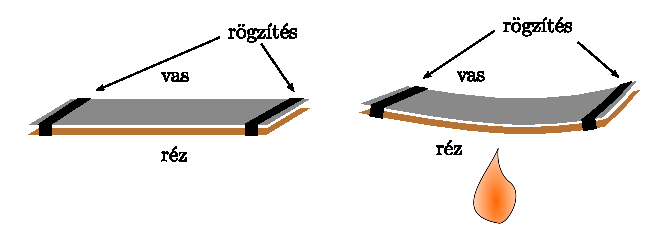
\includegraphics{termo_1/termo_1_6.eps}
        \caption{Bimetál, mely hő hatására elhajlik.}
        \label{fig:termo_1_6}
    \end{figure}.
    \item \emph{Termoelektromos jelenségek:} egyrészt ehhez kapcsolódik, hogy a vezetők ellenállásának is van hőmérsékletfüggése, mely például adott feszültség esetén az áram mérésével meghatározható. Alkalmaznak még termoelemeket is hőmérsékletmérésre. Ebben az esetben két különböző fémet helyeznek egymással kontaktusba, majd különböző hőmérsékletre felfűtik őket (Seebeck\footnote{\,Thomas Johann Seebeck, 1770-1831.}-effektus\footnote{\,Ez a transzportfolyamatok egyik kereszteffektusaként ismert, későbbi tanulmányaitok során az Onsager-relációk kapcsán is találkozni fogtok még vele.}).
    \item \emph{Infrasugárzás:} a test által kibocsátott infrasugárzás mértéke arányos a hőmérsékletével (Planck\footnote{\,Max Planck, 1858-1947.}-féle sugárzási törvény\footnote{\,A Planck-féle sugárzási törvény értelmében az időegység alatt kisugárzott energia: $E\propto T^4$.}). Hőkamera esetében a kamera ezt detektálja, majd színes képpé alakítja. Előnye, hogy a műszer és a mérendő test között nem szükséges a fizikai kontaktus, ezért a műszer egyáltalán nem változtatja meg a mérendő test tulajdonságait.
\end{itemize}
A hőmérsékletméréshez kell egyrészt a mérendő fizikai rendszer, a mérés kalibrációja, illetve referenciapont is. A hőmérsékletmérés feltevései a következők:
\begin{itemize}
    \item a termikus kölcsönhatás miatt a mérendő test és a mérőeszköz hőmérséklete kiegyenlítődik,
    \item a mérőeszköz csak elhanyagolható mértékben változtatja meg a rendszer hőmérsékletét.
\end{itemize}
Fontos megjegyezni még emelett, hogy minden módszer csak bizonyos tartományok között működik (pl.~az alkoholos hőmérők is adott hőmérséklet alatt megfagynak).

Említettük már, hogy hőmérsékleti skálákat lehet definiálni, melyek közül a leggyakoriabbak:
\begin{itemize}
    \item \emph{Celsius-skála:} 1742-ben alkotta meg Celsius. Eredetileg ő 0$^\circ$C-nak a víz forráspontját és 100$^\circ$C-nak a víz fagyáspontját határozta meg standard légköri nyomáson, a köztük lévő részt pedig egyenlő közönként 100 részre osztotta. Ma a skálát pont fordítva használjuk: a víz fagyáspontja 0$^\circ$C, míg a forráspontja 100$^\circ$C normál légköri nyomáson.
    \item \emph{Fahrenheit\footnote{\,Daniel Gabriel Fahrenheit, 1686-1736.}-skála:} 1724-ben alkotta meg Fahrenheit. Olyan hőmérsékleti skálát akart alkotni, ahol nincsenek negatív számok. 0$^\circ$F-nek a szülővárosában, Gda\'nskban, 1708 telén mért leghidegebb hőmérsékletet választotta (ami egy megfelelő telített sósvíz fagyáspontjával könnyen reprodukálható volt), 100$^\circ$F-nek pedig az emberi test normál, 37$^\circ$C-os hőmérsékletét választotta. Ekkor 32$^\circ$F a víz fagyáspontja míg 212$^\circ$F a víz forráspontja standard légköri nyomáson\footnote{\,A Celsius- illetve Fahrenheit-skálák közötti átváltás: $$T_C = \frac 59(T_F -32),\quad  T_F = \frac 95 T_C+32,$$ ahol $T_C$ és $T_F$ jelöli rendre a Celsius- illetve Fahrenheit-skálán mért hőmérsékleteket.}. Ma már csak az angolszász nyelvterületeken használatos.
    \item \emph{Kelvin\footnote{\,Lord Kelvin, Kelvin első bárója vagy William Thomson, 1824-1907.}-skála:} a fizikai számolások szempontjából ez a legfontosabb, a továbbiakban minden hőmérsékleti kifejezést ebben értünk, kivéve ha azt külön nem jelezzük. Ez az \emph{abszolút hőmérsékleti skála}. Az abszolút 0 fok: $0 \mathrm K = -273{,}16^\circ$C. Abszolút 0 fokon a részecskék nem végeznek hőmozgást, azonban a $0$K tetszőlegesen megközelíthető, de nem érhető el\footnote{\,Ezzel a termodinamika III.~főtétele kapcsán még részletesen is fogunk foglalkozni.}. Említettük már korábban, hogy a hőmérsékletméréshez referenciapont is szükséges, ami a Kelvin-skála esetében a $0$K és a víz ún.~hármaspontja\footnote{\,A víz hármaspontjának nevezzük, amikor a hőmérséklet $273{,}1575$K, a nyomás pedig $611{,}657$Pa, ekkor mindhárom halmazállapota (szilárd, folyadék, gáz) egyszerre vannak jelen.}; $1$K hőmérsékletkülönbség a víz hármaspontjának $1/273{,}16$-od része. Ennek megfelelően a két skála közötti átváltás: $T_K = T_C + 273{,}16$, ahol $T_K$ és $T_C$ jelöli rendre a Kelvin- illetve Celsius-skálán mért hőmérsékleteket.
\end{itemize}
A termodinamika tárgyalását könnyen kezelhető rendszerekkel kezdjük. \emph{Egyszerű termodinamikai rendszerről} beszélünk, ha
\begin{itemize}
    \item izotrop: nincs kitüntetett irány,
    \item homogén: nincs kitüntetett pont,
    \item nincsen semmilyen elektromágneses jelenség,
    \item a felületi jelenségek elhanyagolhatóak,
    \item két darab független állapotjelző van.
\end{itemize}
Állapotjelzőnek nevezzük az olyan fizikai mennyiségeket, melyek egy egyszerű termodinamikai rendszer esetén
\begin{itemize}
    \item jellemzik a rendszer makroszkópikus állapotát,
    \item egy állapotban egyértelműen meghatározottak,
    \item nem függenek a rendszer múltjától.
\end{itemize} 
Megjegyezzük, hogy végtelen sok állapotjelző van, ugyanis bármely két állapotjelző kombinációja is állapotjelző. Két csoportba lehet sorolni az állapotjelzőket: az \emph{extenzív állapotjelzők} additívak (összeadódnak), ilyen például a térfogat ($V$), a részecskeszám ($N$), a belső energia ($U$), az entrópia ($S$)\footnote{\,Ezekkel a későbbiekben még részletesen fogunk foglalkozni.}, míg az \emph{intenzív állapotjelzők} egyensúlyban kiegyenlítődnek, függetlenek a rendszer mennyiségétől; ilyen például a nyomás ($p$), a hőmérséklet ($T$) vagy a kémiai potenciál ($\mu$). Az állapotjelzők gyakran nem függetlenek egymástól, a köztük fennálló összefüggéseket \emph{állapotegyenleteknek} nevezzük. Ez utóbbiak tehát az állapotjelzők függvényei, melyek minden esetben az alábbi alakban írhatóak fel:
\begin{align}
    f(p,V,T,\dots)=0.
\end{align}
Az állapotegyenlet meghatározása alapvetően kísérleti úton történik és a vizsgált anyagra jellemző\footnote{Később meghatározható lesz a statisztikus fizika módszereivel is.}.

\emph{Termodinamikai egyensúlyról} beszélünk, ha a rendszer makroszkopikus tulajdonságai, és ezáltal az állapotjelzői időben állandóak. Legyen három rendszerünk, jelöljük őket A, B és C-vel. Fontos megállapítás, hogy ha A és B rendszer, illetve B és C rendszer is egyensúlyban vannak, akkor A és C rendszer is egyensúlyban vannak egymással, azaz ha termikus kapcsolatba kerülnek, akkor az nem okozza az állapotjelzők megváltozását. Ezt az axiómát hívjuk a \emph{termodinamika 0.~főtételének}.

Az egyik legfontosabb egyszerű termodinamikai rendszer az ún.~\emph{ideális gáz}. Ideális gázról beszélünk, ha:
\begin{itemize}
    \item a gázt alkotó atomok vagy molekulák térfogata a gáz által kitöltött térfogathoz képest elhanyagolható,
    \item a gázmolekulák egymással ütköznek, azonban más (taszító vagy vonzó) kölcsönhatásban egymással nem állnak,
    \item a gázmolekulák egymással illetve a fallal vett ütközése tökéletesen rugalmas,
    \item a gázmolekulák átlagos sebességét és kinetikus energiáját a gáz hőmérséklete szabja meg valamint
    \item az azonos hőmérsékleten, azonos számú gázmolekula kinetikus energiája megegyezik, és független a gáz anyagi minőségétől.
\end{itemize}
Három fontos kísérlet és ebből levont következtetés vonatkozik az ideális gázokra, melyekből az állapotegyenlete meghatározható.
\begin{itemize}
    \item \emph{Boyle\footnote{\,Robert Boyle, 1627-1691.}--Mariotte\footnote{\,Edme Mariotte 1620-1684.}-törvény:} 1669-ben fogalmazták meg, hogy állandó hőmérsékleten $pV = \textnormal{konst.}$, azaz a nyomás és a térfogat fordítottan arányosak egymással. Ennek igazolásához különböző nyomások mellett mérjük, hogy egy csőben lévő golyó mennyivel mozdul el, azaz hogyan változik meg a bezárt levező térfogata, ez látható \aref{fig:termo_1_4}. ábrán.
    \item \emph{Gay-Lussac\footnote{\,Joseph Louis Gay-Lussac, 1778-1850.} I.~törvénye:} 1802., állandó nyomáson melegítés hatására nő a gáz térfogata, mégpedig a hőmérséklet és a térfogat megváltozása között egyenes arányosság áll fent. Továbbá igaz, hogy:
    \begin{align}
        V(t) = V_0(1+\beta t),
    \end{align}
    ahol $V$ a térfogat, $V_0$ a $0^\circ$C-on mért térfogat, $\beta$ az ún.~térfogati hőtágulási együttható, $t$ pedig a $^\circ$C-ban mért hőmérséklet. \Aref{fig:termo_1_1}. ábrán látható, hogy a térfogat a hőmérsékletnek lineáris függvénye. 
    \begin{figure}[h!]
    \centering
    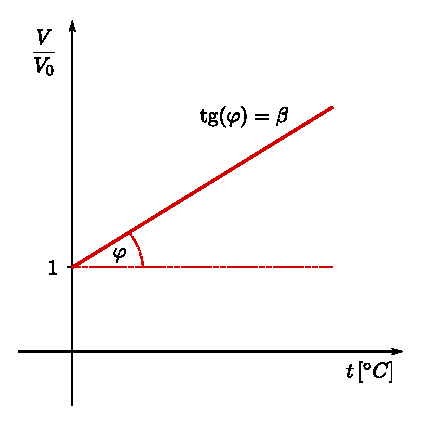
\includegraphics{termo_1/termo_1_1.eps}
    \caption{Gay-Lussac I. törvénye.}
    \label{fig:termo_1_1}
    \end{figure}
Ennek a méréséhez manométer segítségével mérjük különböző hőmérsékleteket a bezárt levegő térfogatának változását, mely során az U-alakú csőben lévő folyadékoszlop elmozdul. A kísérleti összeállítás látható \aref{fig:termo_1_5}. ábrán.
    \begin{figure}[!h]
    \centering
    \begin{subfigure}[t]{0.45\textwidth}
            \centering
            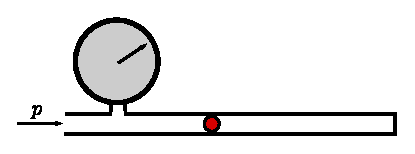
\includegraphics[width=\textwidth]{termo_1/termo_1_4}
            %\phantonsubcaption
            \newsubcap{Boyle--Mariotte-törvény kimérése}
            \label{fig:termo_1_4}
    \end{subfigure}\hfill
    \begin{subfigure}[t]{0.45\textwidth}
            \centering
            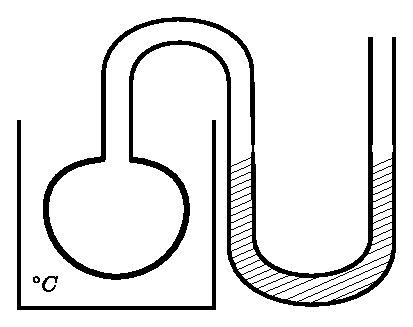
\includegraphics[width=\textwidth]{termo_1/termo_1_5}
            \newsubcap{Gay-Lussac I. törvényének mérési elrendezése}
            %\phantomsubcaption
            \label{fig:termo_1_5}
    \end{subfigure}
    \phantomcaption
    \end{figure}
    \item \emph{Gay-Lussac II.~törvénye:} Állandó térfogaton melegítés hatására nő a gáz nyomása. A hőmérséklet és a nyomás között egyenes arányosság áll fent. Igaz, hogy:
    \begin{align}
        p(t) = p_0(1+\beta t),
    \end{align}
    ahol $p$ a nyomás, $p_0$ pedig a $0\,^\circ$C-on mért nyomás. Fontos megállapítás, hogy a Gay-Lussac I.~és II.~törvényében megjelenő $\beta$ ugyanaz, értéke pedig a kísérletek alapján $\beta = 1/273{,}16\, ^\circ\mathrm C$. Ez igaz minden ideális gázra (a hélium például nagyon jó közelítéssel ideális gáznak tekinthető).
\end{itemize}
Ezek alapján az ideális gáz állapotegyenletét már meghatározhatjuk az alábbi gondolatkísérlettel. Induljunk ki egy $0\,^\circ\text C$-os ideális gázból, melynek térfogata $V_0$, nyomása pedig $p_0$. Először állandó nyomáson növeljük meg a hőmérsékletét $t$-re, majd állandó hőmérsékleten a térfogatát változtassuk $V$-re. Így tetszőleges $t$ és $V$ elérhető. A folyamatot lásd \aref{fig:termo_1_2}. ábrán.
A fenti törvények alapján ekkor:
\begin{align}
    \begin{array}{rcl} V_1\hspace{-2mm} &=& \hspace{-2mm}V_0(1+\beta t)\\ \quad p_0V_1 \hspace{-2mm}&=&\hspace{-2mm} pV\end{array}  \quad\Rightarrow\quad pV = p_0V_0(1+\beta t)=\underbrace{p_0V_0\beta}_{\substack{=nR,\\\textnormal{ez mérhető}}}\hspace{-2mm} T\quad\Rightarrow\quad pV = nRT,
\end{align}
ahol $T = t+1/\beta$ a Kelvinben mért hőmérséklet, $n$ jelöli az anyagmennyiséget\footnote{\,A mértékegysége $[n] = \textnormal{mol}$, 1 mol a 12 g $^{12}$C-ben lévő atomok száma.}, $R=8{,}314 \text{ J}/\left(\text{mol K}\right)$ az univerzális gázállandó. Az $n$ anyagmennyiség meghatározható egyrészt az Avogadro\footnote{\,Amadeo Avogadro, 1776-1856.}-állandó ($N_A \approx 6\cdot 10^{23}$) segítségével és az összes részecske számával mint $n = N/N_A$, illetve ha ismert a teljes rendszer tömege ($m$), illetve a moláris tömeg ($M$), akkor $n = m/M$. \Aref{fig:termo_1_3}. ábrán látható, hogy tényleg Kelvin-skálára áttérve 0K-en lesz a gáz térfogata zérus.
\begin{figure}[!h]
    \centering
    \begin{subfigure}[t]{0.45\textwidth}
            \centering
            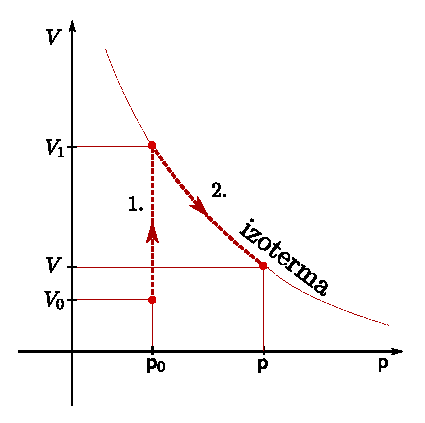
\includegraphics[width=\textwidth]{termo_1/termo_1_2}
            \newsubcap{Folyamat a $\pres-V$ síkon, melyből az állapotegyenlet meghatározható.}
            \label{fig:termo_1_2}
    \end{subfigure}\hfill
    \begin{subfigure}[t]{0.45\textwidth}
            \centering
            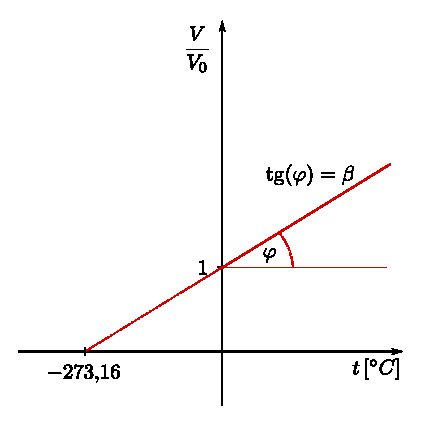
\includegraphics[width=\textwidth]{termo_1/termo_1_3}
            \newsubcap{Kelvin-skálára áttérve 0K-en lesz a gáz térfogata zérus, az egyenes meredeksége pedig pont $\beta$.}
            \label{fig:termo_1_3}
    \end{subfigure}
    \end{figure}
Az előzőek alapján az ideális gáz állapotegyenlete tehát:
\begin{align}
    pV = nRT.
\end{align}